% Change 'digital' to 'printed' before printing
\documentclass[
  digital, %% This option enables the default options for the
           %% digital version of a document. Replace with `printed`
           %% to enable the default options for the printed version
           %% of a document.
  table,   %% Causes the coloring of tables. Replace with `notable`
           %% to restore plain tables.
  lof,     %% Prints the List of Figures. Replace with `nolof` to
           %% hide the List of Figures.
  lot,     %% Prints the List of Tables. Replace with `nolot` to
           %% hide the List of Tables.
  oneside,
  %% More options are listed in the user guide at
  %% <http://mirrors.ctan.org/macros/latex/contrib/fithesis/guide/mu/fi.pdf>.
]{fithesis3}
%% The following section sets up the locales used in the thesis.
\usepackage[resetfonts]{cmap} %% We need to load the T2A font encoding
\usepackage[main=english, slovak]{babel}

%% For non-Latin scripts, it may be necessary to load additional
%% fonts:
\usepackage{paratype}
%%
%% The following section sets up the metadata of the thesis.
\thesissetup{
    date          = 2017/5/22,
    university    = mu,
    faculty       = fi,
    type          = mgr,
    author        = Zuzana Dankovčíková,
    gender        = f,
    advisor       = Bruno Rossi PhD,
    title         = {Custom Roslyn Tool for Real-Time Static Code Analysis},
    TeXtitle      = {Custom Roslyn Tool for Real-Time Static Code Analysis},
    keywords      = {roslyn, C\#, compilers, code review, .NET compiler platform, Kentico, analyzer, code fix...},
    TeXkeywords   = {roslyn, C\#, compilers, code review, .NET compiler platform, Kentico, analyzer, code fix..., \ldots},
}
\thesislong{abstract}{
    TODO: This is the abstract ...
}
\thesislong{thanks}{
    TODO: This is the acknowledgement\dots

}

%% The following section sets up the bibliography.
\usepackage{csquotes}
\usepackage[              %% When typesetting the bibliography, the
  backend=biber,          %% `numeric` style will be used for the
  style=numeric,          %% entries and the `numeric-comp` style
  citestyle=numeric-comp, %% for the references to the entries. The
  sorting=none,           %% entries will be sorted in cite order.
  sortlocale=auto         %% For more unformation about the available
]{biblatex}               %% `style`s and `citestyles`, see:
%% <http://mirrors.ctan.org/macros/latex/contrib/biblatex/doc/biblatex.pdf>.
\addbibresource{mybib.bib} %% The bibliograpic database within
                          %% the file `example.bib` will be used.

\usepackage{makeidx}      %% The `makeidx` package contains
\makeindex                %% helper commands for index typesetting.

%% These additional packages are used within the document:
\usepackage{paralist}
\usepackage{amsmath}
\usepackage{amsthm}
\usepackage{amsfonts}
\usepackage{url}
\usepackage{menukeys}

\begin{document}
% =================================================================
% ============================= CHAPTER 1 =========================
% =================================================================
\chapter{Introduction}
TODO...

Ideas:

What is code quality, why is it important, tool that support it.. compilers, diversion ... aaaand here comes Roslyn which provides compiler as a platform.  

In~the~.NET world, the~compiler used~to~be a~black box that given the~file paths to~the~source text, produced an~executable (see Figure~\ref{fig:compiler-as-a-black-box}). In~order~to do that, compiler has to collect large amount of~information about the~code it is processing. This knowledge, however, was unavailable to~anyone but the~compiler itself and it was immediately forgotten once the~translated output was produced~\cite{roslyn-overview-github}. 

Why is this an~issue when for decades this black-boxes served us well? Programmers are increasingly becoming reliant~upon the~powerful integrated development environments (IDEs). Features like IntelliSense, intelligent rename, refactoring or~"Find all references" are key~to~developers' productivity; and~even more so in~an~enterprise-size systems. 

This gave a~rise to~number of~tools that analyze the~code for common issues and are able to~suggest a~refactoring. The problem is that that such~tool needs to~parse the~code first in~order~to be~able~to~understand and~analyze it. As a result companies need to invest fair amount of resources to duplicate the logic that the .NET compiler already possesses. Not only is it possible that the compiler and the tool may disagree on some specific piece of code, but with every new version of C\# the tool needs to be updated to handle new language features\cite{dot-net-development-using-the-compiler-api}.

With roslyn.. etc. etc. .. API for analysis.. use in companies for custom analyzers... etc. etc....
 https://github.com/dotnet/roslyn/wiki/Roslyn Overview -- motivation
Make sure to stress out that ".NET Compiler Platform" and "Roslyn" names will be used interchangably as it is in Roslyn Succinctly on page 11.
% =================================================================
% ============================= CHAPTER 2 =========================
% =================================================================
  \chapter{Code Quality and Static Code Analysis}
TODO

% =================================================================
% ============================= CHAPTER 3 =========================
% =================================================================
  \chapter{.NET Compiler Platform}
As~per~\cite{dragon-book}, compiler is a~program that can read a~program in a~\textit{source} language and~translate it into an~equivalent program in~\textit{target} language while reporting any errors detected in~the~translation process. 

In~the~.NET world, the~compiler used~to~be a~black box that given the~file paths to~the~source text, produced an~executable (see Figure~\ref{fig:compiler-as-a-black-box}). This perception was changed in~2015 when Microsoft introduced the .NET Compiler Platform (commonly referred to as "Project Roslyn").  

\begin{figure}[h!]
		\centering
			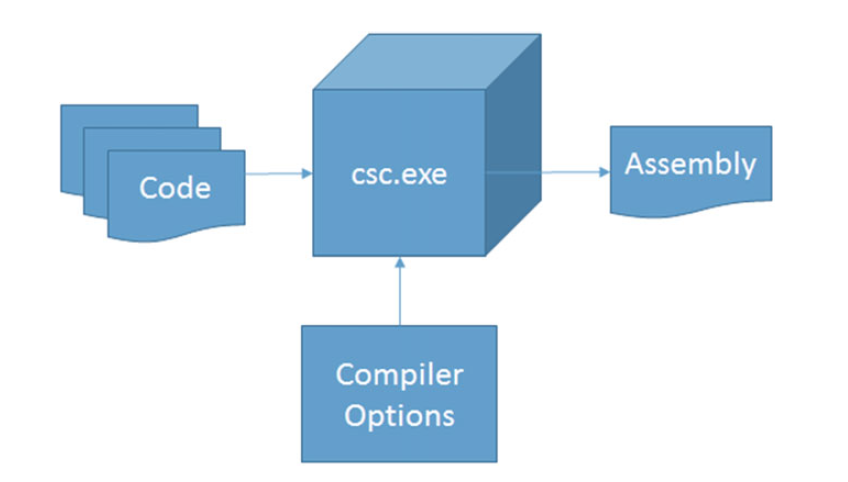
\includegraphics[scale=0.35]{img/compiler-as-a-black-box}
		\caption{Compiler as a black box\cite{dot-net-development-using-the-compiler-api}}
		\label{fig:compiler-as-a-black-box}
\end{figure}

Not only have been compilers for both VisualBasic and C\# rewritten into entirely managed code, they also expose the internals of the compiler pipeline via a public .NET API~\footnote{Application Programming Interface}. This makes them a platform (also known as \textit{compiler-as-as-service}) with rich code analysis APIs that can be leveraged by developers to perform analysis, code generation or dynamic compilation in their own programs~\cite{roslyn-succinctly}. Those can be later easily integrated into VisualStudio all without the hard work of duplicating compilers' parsing logic.

This chapter will take a look at how the Roslyn API layers are structured, how the original source code is represented by the compiler and how developers can build tools upon the compiler's API. Lastly it will provide a short overview and evaluation of other tools that were used before Roslyn or have emerged thanks to .NET Compiler Platform.

Note that although Roslyn provides equivalent APIs for both VisualBasic and C\#, this thesis will only focus on the C\# part, since only that one is relevant for the practical part of the thesis.
  
  
  \section{Compiler APIs}
  
  \section{Syntax Tree API}
  \section{Semantics API}
  \section{Workspaces API}
  
%  - how to perform static code analysis with Roslyn
%    - writing anlyzers and code fixes / code refactorings  
  
  \section{Other Tools}
  %3. Other tools for code analysis available for C#
%  - new DotNetAnalyzers available thanks to Roslyn
%  - Resharper,
%  - FxCop
%  - StyleCop

% =================================================================
% ============================= CHAPTER 4 =========================
% =================================================================

% =================================================================
% =============================== STUFF ===========================
% =================================================================
	% From template
	\makeatletter\thesis@blocks@clear\makeatother
	\phantomsection %% Print the index and insert it into the
	\addcontentsline{toc}{chapter}{\indexname} %% table of contents.

	\printindex
    
% =================================================================
% =========================== BIBLIOGRAPHY ========================
% =================================================================
    \printbibliography

% =================================================================
% ============================ APPENDICES =========================
% =================================================================    
	\appendix %% Start the appendices.
  \chapter{Upgrades and Versioning}
TODO...

\end{document}
